This chapter will describe how we implemented the simulator. The simulator consists of multiple parts: \\
\begin{enumerate}
	\item Parsing
	\item Contextual Analyzing
	\item Simulation
\end{enumerate}

The following figure \ref{fig:scripttosimu} shows the process from script files to output on the screen.

\begin{figure}[H]
\centering
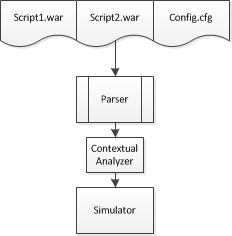
\includegraphics[scale=1.2]{rapport/6/figures/script_to_simu}
\label{fig:scripttosimu}
\caption{From scripts to simulation}
\end{figure}

\section{Parser construction}
	The job of a parser is to check if a program is syntactically correct and 
	to determine the structure of the program (Here we constructed an {\it abstract syntax tree} - see section \ref{ast}).
	A parser can only read {\it tokens}, which is terminals as seen in the EBNF. So before we are able to parse we need to convert 
	the program code from characters to tokens, this is done by using a scanner, that will be explained next. Beside having a scanner it is 
	also important to choose a strategy for parsing, which we will look at in \ref{impl:parsestrats}.
	
	\subsection{Scanner}
		The scanner, also called a lexer, is used to convert text in the text files to tokens. 
		It reads a text file as a stream of characters and tries to identify which token it is currently reading.
		To identify tokens a table with the correct spellings of tokens is used.			 
		
	\subsection{Parse Strategies}
		\label{impl:parsestrats}
		A parse strategy is, beside checking that the code is syntactically correct a way to build our AST. 
		To determine which production rule the parser is currently reading, 
		a parser is using {\it lookahead}, which is a number representing how many tokens we have to look at, 
		at a time to determine the production rule.
		There are two common strategies for parsing code, called {\it Bottom-up Parsing} and {\it Top-Down Parsing}, that are explained next.
	\paragraph{Bottom-up Parsing}
		This way of parsing takes simple structures and combining them to more complex structures.
		This type of parsing is commonly called {\it LR parsing} because we read the text from the left and reduces to the right.
		A LR parser with $k$ lookahead is called a LR($k$) parser.
		\begin{figure}[H]
			\centering
			\subfloat[Top down]{\label{fig:top_down}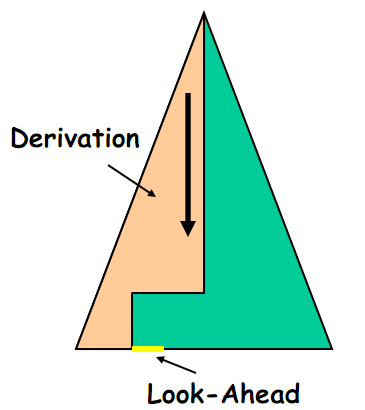
\includegraphics[width=0.4\textwidth]{rapport/6/figures/topdown}} 
			\subfloat[Bottom up]{\label{fig:bottom_up}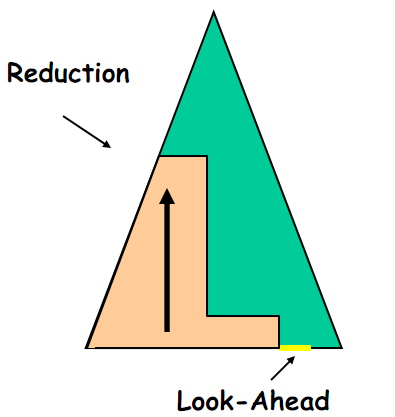
\includegraphics[width=0.4\textwidth]{rapport/6/figures/bottomup}}
			\caption{Two different parse strategies:Top-down(LL) on the left and bottom-up(LR) on the right}\label{fig:parsers}
		\end{figure}
		
	\paragraph{Top-down Parsing}
		Top-down parsing figure \ref{fig:top_down} starts from the complex structures, and breaks them down into smaller parts.
		This type of parsing is commonly called {\it LL parsing} because we read the text from the left and make derivations to the left.
		A LL parser with $k$ lookahead is called a LL($k$) parser.
	\paragraph{Strengths and weaknesses}
		The most commonly used parsing strategy of the two is LR parsing, the reason for this is because it is faster than LL parsing.
		In this project, however we have chosen to make a LL parser because it is easy to implement, furthermore speed is not important for us. 
		The type of LL parser we made is called a recursive descent parser, which can parse LL(1) grammars.
		
	\subsection{Abstract Syntax Tree}
		\label{ast}
		The structure of the parsed program is stored as an AST. The tree structure is called abstract because it does not contain the concrete
		structure of the EBNF, but rather an abstract representation of the source code. Because of this there is not a straightforward way to 
		construct such a tree.  We constructed the AST-structure by making a class for each of the node we wanted represented, i.e. we have 
		classes for expressions, declarations and different datatypes. \\
		
		Compared to the EBNF the AST is more specific i.e. an Expression 
		is not simply an Expression, but it can be an {\it IntegerExpression} or a {\it RegimentStatExpression}. 
		To make parsing easier we use polymorphism so that all variants of an expression 
		will inherit from the class Expression and likewise for similar constructs. 
		Furthermore all classes which are not a subtype of another, inherit from a class called {\it AST}, 
		the reason for this will be explained in section \ref{impl:visitor}, which is the only place we directly use it.
		
		\paragraph{Small example}
			Here is a small example of how an AST could look like when parsing our code.
			\begin{figure}[H]
			\center
			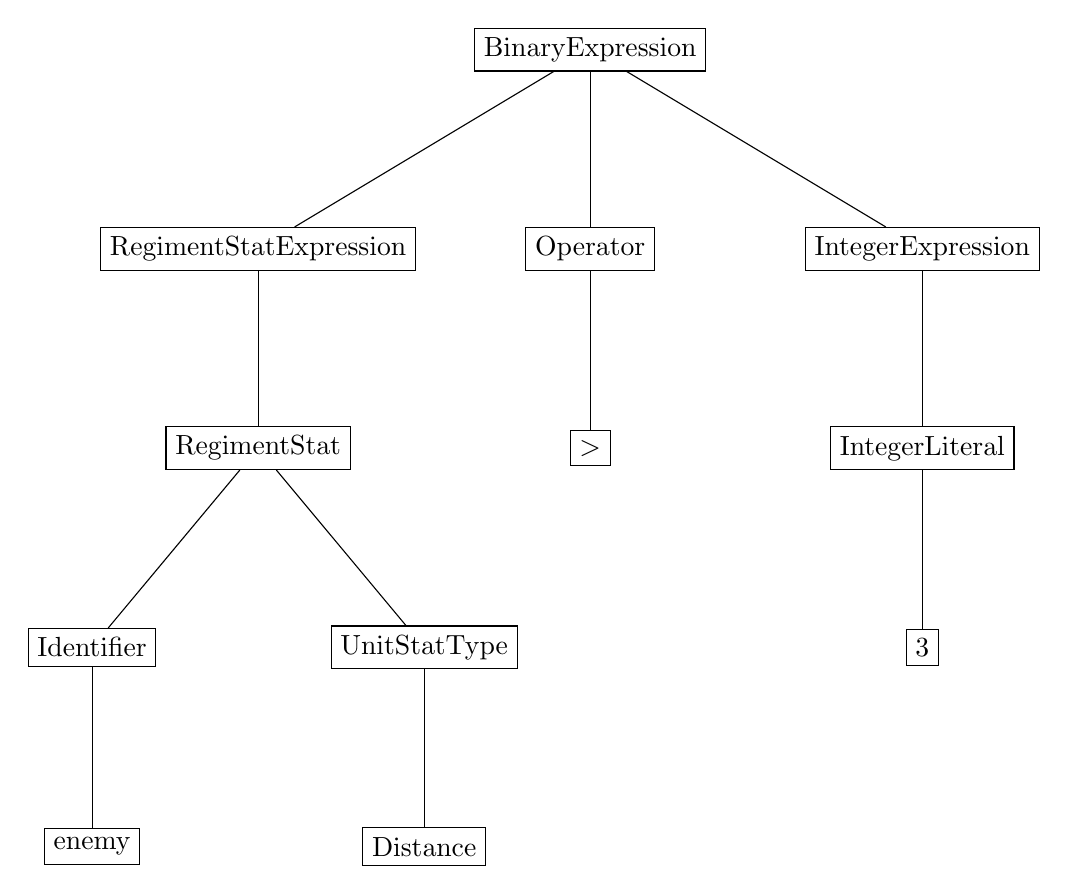
\begin{tikzpicture}[sibling distance=120pt]
			    \tikzstyle{every node}=[draw,rectangle]
			    \tikzset{level distance=72pt}
			    \node {BinaryExpression}
			        child 
			        { 
			        	node {RegimentStatExpression} 
			        		child
			        		{ 
			        			node {RegimentStat}
			        			child
			        			{
			        				node{Identifier}
			        				child{node{enemy}}
			        			}
			        			child
			        			{
			        				node{UnitStatType}
			        				child{node{Distance}}
			        			}
			        		}
			        }
			        child 
			        {
			            node {Operator}
			            child { node {$>$} }
			        }
			        child 
			        { 
			        	node {IntegerExpression} 
			        	child 
			        	{ 
			        		node {IntegerLiteral}
			        		child{node {3}}
			        	}
			        }
			        ;
			\end{tikzpicture}
			\caption{AST of a binary expression}
			\end{figure}
			The tree shows an AST of a {\it BinaryExpression}. 
			The tree is equavivalent to the code:
			\begin{verbatim}
				enemy.Distance > 3
			\end{verbatim}
			where {\it enemy} is an identifier, which have been assigned to a regiment.
		How we constructed such a tree in the code is explained in \ref{parsemethods}.
			
	\subsection{Recursive descent parser}
		A recursive descent parser is a LL parser which works by recursively going through the program code.
		The parser we made is a LL(1) parser.
		To construct this type of parser the following is required:
		\begin{enumerate}
			\item EBNF
			\item A scanner for reading chars and identifying them as terminals.
			\item A parse method for each non-terminal in the EBNF.
			\item A method or multiple methods that can accept terminals.
			\item In each of the parse methods accept tokens and call other parse methods, as required.
		\end{enumerate}		 
		
		\subsubsection{Accepting terminals}
			The parser uses an accept method to check if the current token is the token that was expects, if not an error is given.
			The following example shows the {\it Accept method} from our Parser.
			\begin{lstlisting}[basicstyle=\small\sffamily,
					keywords={break,case,const,continue,default,else,enum,
					for,if,return,switch,while,do,long,void,int,float,double,
					char,struct,typedef,include,size\_t},
					keywordstyle={\color{blue}},
					comment={[l]{//}}, morecomment={[s]{/*}{*/}}, commentstyle=\itshape,
					columns={[l]flexible}, numbers=left, numberstyle=\tiny,
					frameround=fftt, frame=shadowbox, captionpos=b,
					caption={Accept method for accepting tokens},
					label=impl:accept]
private void Accept(Token.TokenType expectedType)
{
	if (currentToken.type == expectedType)
    {
		currentToken = scanner.Scan();
    }
    else
    {
    	errorReporter.ReportParserError("Expected " + 
    		expectedType + ", but got " + currentToken.type, currentToken);
    }
}
			\end{lstlisting}
			This method checks if the expected token matches the current token, and then retrieve the next token from the scanner, if it was a match.
			If there is a mismatch, an error will be reported.
			
		\subsubsection{Parse methods}
			\label{parsemethods}
			The parse methods perform in a mutual recursive way, where a parse methods representing the higher level nodes in an 
			AST calls parse methods representing its children. When a lower level node is done parsing it returns this node to a higher level node. This way an AST will be constructed. \\
			Here is a parse method from our code:
			\begin{lstlisting}[basicstyle=\small\sffamily,
					keywords={break,case,const,continue,default,else,enum,
					for,if,return,switch,while,do,long,void,int,float,double,
					char,struct,typedef,include,size\_t},
					keywordstyle={\color{blue}},
					comment={[l]{//}}, morecomment={[s]{/*}{*/}}, commentstyle=\itshape,
					columns={[l]flexible}, numbers=left, numberstyle=\tiny,
					frameround=fftt, frame=shadowbox, captionpos=b,
					caption={Parse method for RegimentDeclarationCommand},
					label=impl:regdeccmd]
private SingleCommand ParseRegimentDeclarationCommand()
{
    Accept(Token.TokenType.Regiment);
 	Identifier i = ParseIdentifier();
  	Accept(Token.TokenType.Assignment);
    RegimentSearch rs = ParseRegimentSearch();
    Accept(Token.TokenType.SemiColon);
	RegimentDeclaration rd = new RegimentDeclaration(i, rs);
	return new RegimentDeclarationCommand(rd,previousTokenPosition);
}
			\end{lstlisting}
			The method is for parsing {\it RegimentDeclarationCommand}s, which consists of a {\it RegimentDeclaration node}.
			The method starts by trying to accept the token {\it Regiment} because a {\it RegimentDeclaration node} must start with this. 
			After this it expects there to be an {\it Identifier node}, which it tries to parse. After the rest of the accepting and parsing the new 
			{\it RegimentDeclarationCommand node} is returned.
		
		